% -----------------------------------------------
\section{Statistical Foundations of PFNs}
% -----------------------------------------------
\begin{frame}{Statistical Foundations of PFNs}
  \framesubtitle{Studied Questions}
  \begin{itemize}
    \item<alert@1> When PPDs can Learn?
    \item<alert@2> How PFNs approximate PPDs?
    \item<alert@3> Why PFNs can learn?
    \item<alert@4> Which ICL properties do transformers (in particular TabPFN) have?
  \end{itemize}
  \note<1>{Since PPDs are the main motivation behind PFNs, they first ask when a PPD can learn from training data.}
  \note<2>{}
  \note<3>{Why can a pre-trained network still learn in the inference phase? 
           Although we know now why a PPD does, a PFN is not a valid PPD, 
           and it is only trained to approximate the PPD for limited training sizes.}
  \note<4>{}
\end{frame}

\begin{frame}[label=ppdlearn]{Statistical Foundations of PFNs}
  \framesubtitle{When PPDs can Learn}
  \small
  \setlength{\abovedisplayskip}{4pt}\setlength{\belowdisplayskip}{4pt}
  \setlength{\abovedisplayshortskip}{2pt}\setlength{\belowdisplayshortskip}{2pt}

  Let $\mathcal{S} = \{\varphi \in \Phi : \mathbb{P}_\Phi(\varphi) > 0\}$ be the \emph{support} of the prior.

  \vspace{-0.2em}
  \begin{block}{Theorem 3.1 (Posterior consistency). \cite{naglerStatisticalFoundationsPriorData2023}}
    Under \hyperlink{ppdlearn<2>}{\textcolor{blue!55!black}{\emph{some}}} assumptions, there exists $\varphi^* \in \mathcal{S}$ such that for almost every $(y, x)$,
    \[
      \pi(y \mid x, \mathcal{D}_n) \;\xrightarrow[\;n \to \infty\;]{}\; \varphi^*(y \mid x) \qquad \text{a. s.}
    \]
    and $\varphi^*$ is the KL-optimal approximation of $p_0$ in $\mathcal{S}$:\quad
    $\displaystyle \varphi^* = \arg\min_{\varphi \in \mathcal{S}} \mathrm{KL}\big(\varphi \,\|\, p_0\big).$
  \end{block}

\end{frame}

\begin{frame}{Statistical Foundations of PFNs}
  \framesubtitle{PFN Approximation of the PPD}
  % content
\end{frame}
\begin{frame}{Statistical Foundations of PFNs}
  \framesubtitle{Bias-Variance Decomposition of PFNs}
  % content
\end{frame}

\begin{frame}{Statistical Foundations of PFNs}
  \framesubtitle{Variance and Diminishing Sensitivity}
  % content
\end{frame}

\begin{frame}{Statistical Foundations of PFNs}
  \framesubtitle{Bias and the Need for Locality}
  % content
\end{frame}

\begin{frame}{Statistical Foundations of PFNs}
  \framesubtitle{Transformer Networks}
  % content
\end{frame}

\begin{frame}{Statistical Foundations of PFNs}
  \framesubtitle{Localized PFNs}
  % content
\end{frame}


\begin{frame}{Statistical Foundations of PFNs}
  \framesubtitle{Numerical Validation}
  \begin{figure}
    \centering
    % 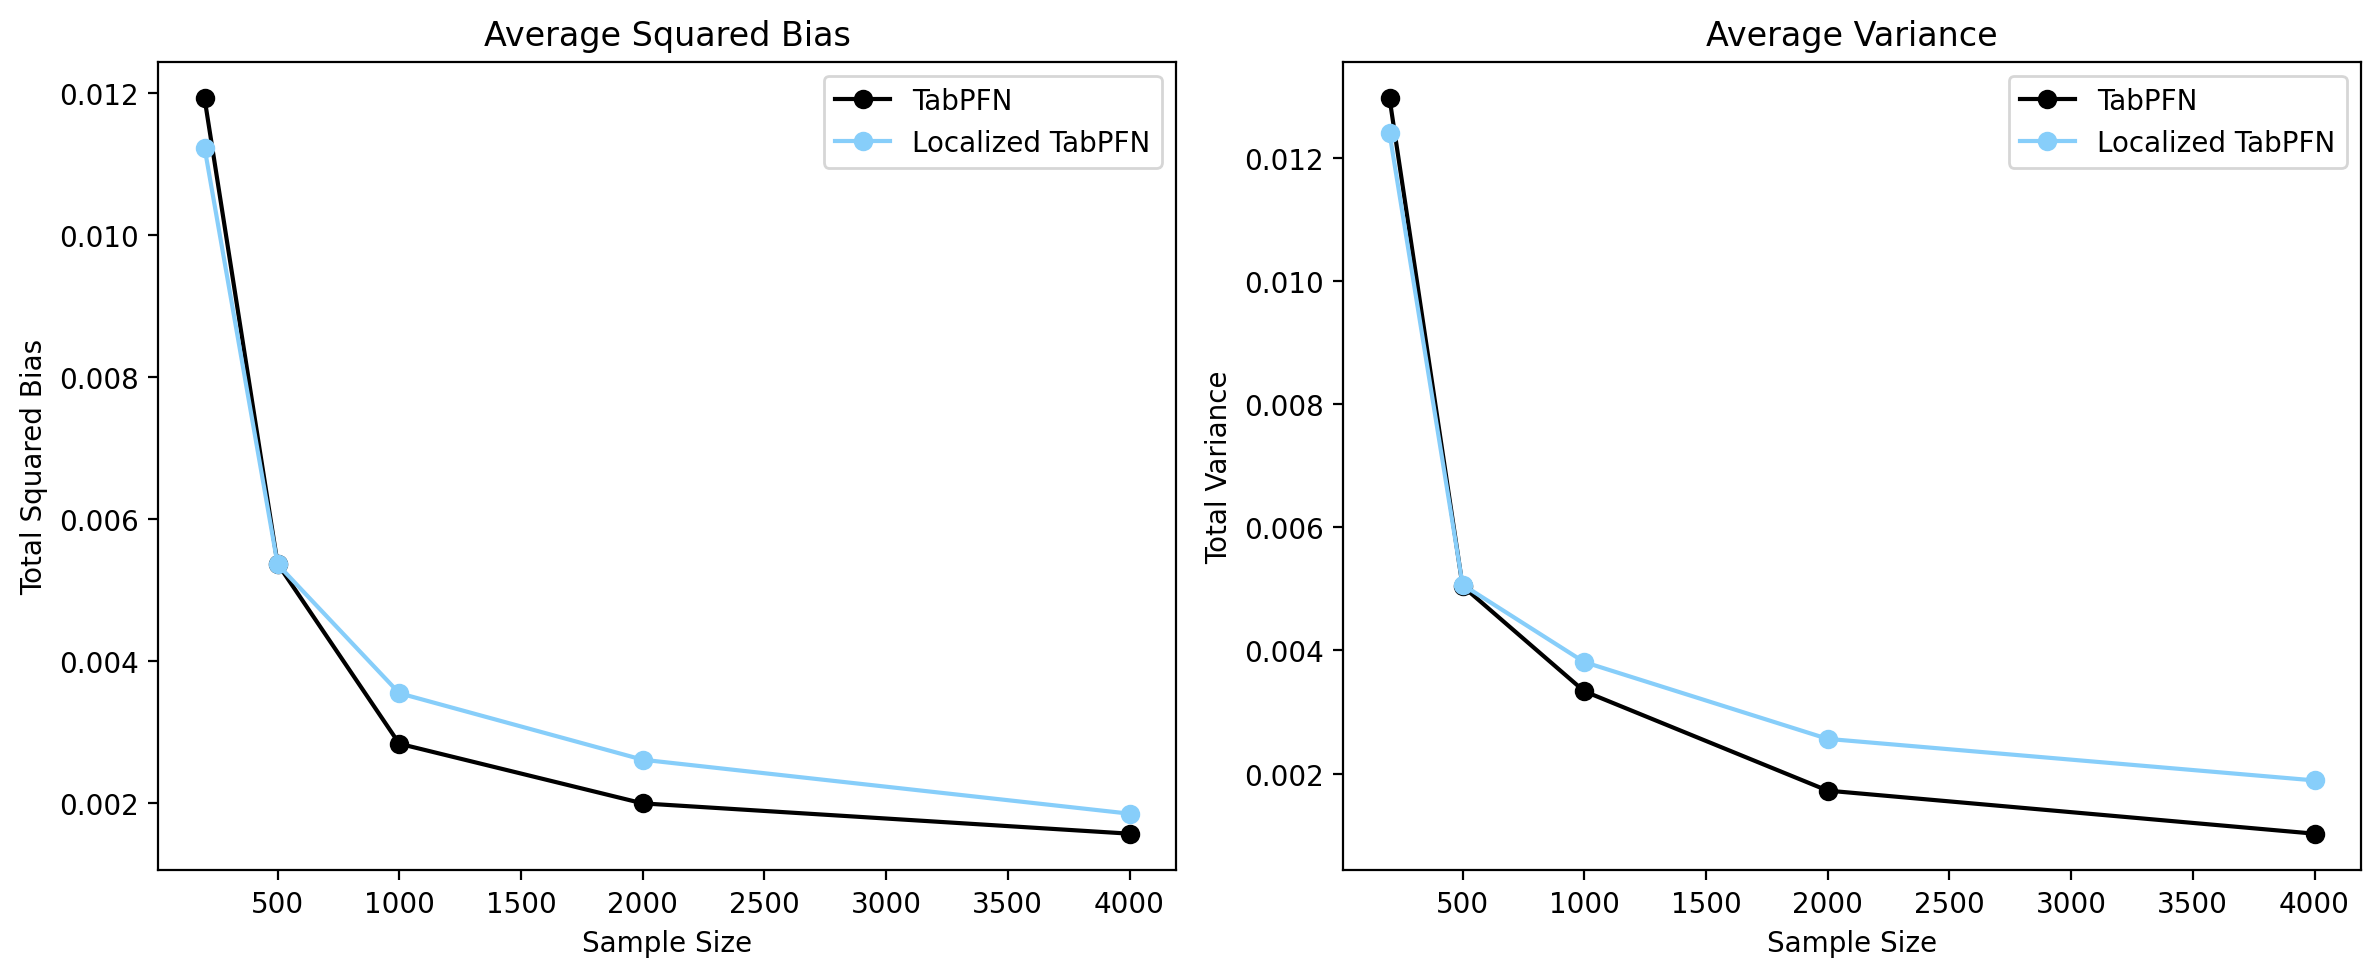
\includegraphics[width=0.8\linewidth]{../src/results/bias_variance_plot_v3.png}
    \caption{Caption here.}
  \end{figure}
\end{frame}

\begin{frame}{Statistical Foundations of PFNs}
  \framesubtitle{Discussion}
  % content
\end{frame}
